In this chapter, we begin by presenting the experimental datasets, CIFAR10 and CIFAR100 along with the image feature extraction process. Next we adapt three methods overviewed in Chapter \ref{bg} to reduce the size of image dataset, called the Patterns by Ordered Projections (POP) \cite{Riquelme2003a}, Enhanced Global Density-based Instance Selection (EGDIS) \cite{Malhat2020}, and Curriculum Learning (CL) \cite{Hacohen2019a}. Then we propose our edited data reduction method, called Weighted Curriculum Learning (WCL), based on CL scores and Boundary Based Curriculum Learning (BBCL), based on the EGDIS selected boundary instances. After that, our work is focused on the comprehensive evaluation of the methods. We illustrate the data reduction geometry patterns with three generated datasets, blobs, moons and circles. We then describe the model fitting procedure of the logistic regression algorithm. Finally, we extend the reduction pipeline to deep learning method with the particular network, DenseNet121. Figure \ref{Fig.reduction_pip} gives the pipeline overview of this project.  

 \begin{figure}[H]
 \centering
 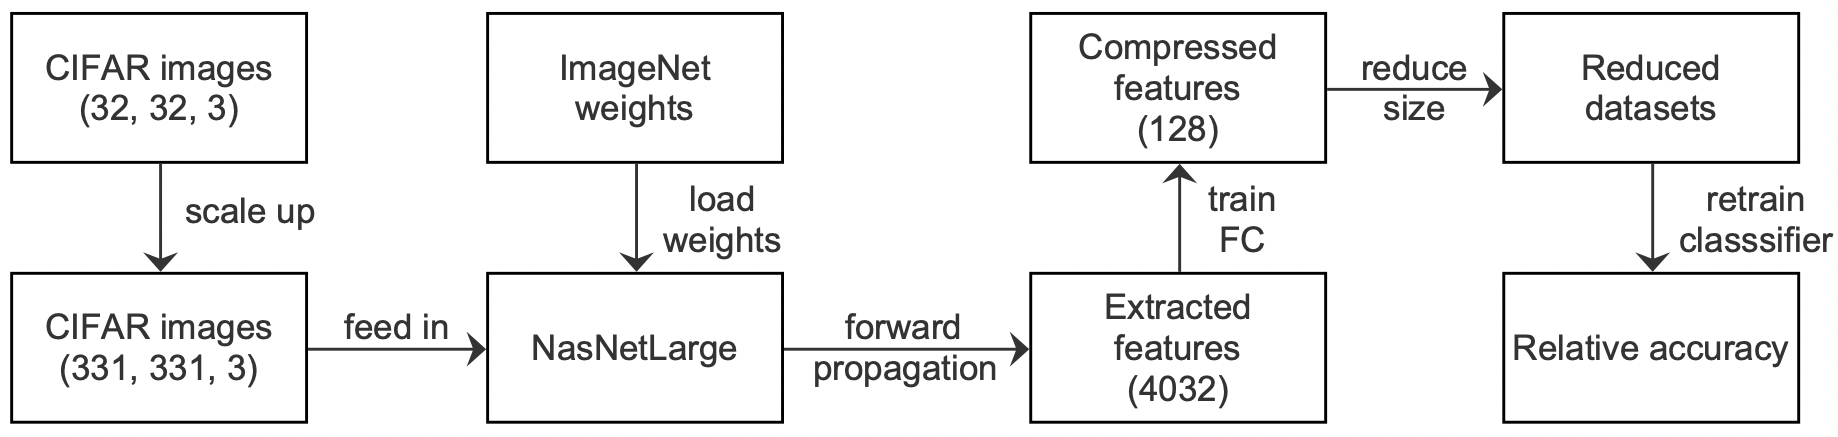
\includegraphics[width=1\textwidth]{src/pipeline.png}
 \caption{Overview of the data reduction pipeline.}
 \label{Fig.reduction_pip}
 \end{figure}

\section{Datasets and Image Feature Extraction}
We choose to use CIFAR10 and CIFAR100 \cite{Krizhevsky2009} as our experimental datasets which contain 6,000 and 600 tiny images of size 32$\times$32 per class respectively. The advantage of CIFAR is that they are large in the number of images and small in the size of images. With CIFAR datasets, we could train the network faster thus explore the reduction rate for a wider scale within the required timetable. Another advantage is that CIFAR datasets can reflect the performance of data reduction algorithms for both simple dataset and hard dataset in term of classification accuracy. According to Kornblith et al. \cite{Kornblith2018}, the test set results indicate that CIFAR10 is very easy to classify and CIFAR100 is as difficult as other high resolution datasets such as the Describable Textures Dataset (DTD) \cite{Cimpoi2014}, Food-101 \cite{Bossard2014}. These features could gain us thorough and representative evaluation results with limited compute resources.

After scaling up the image size to 331 and transforming the images into range 0 to 1 by dividing 255, we therefore performed the feature extraction task. The goal was to provide structural data for the data reduction algorithms to work with. We did this job with pre-trained NasNetLarge \cite{Zoph2018} because Kornblith et al. \cite{Kornblith2018} have evaluated the quality of extracted features and the quality of extracted features is good enough. Their experiments show that the classification scores with simple logistic regression are very close to the state-of-art classification scores with CNN. In order to simplify the implementation, we chose to use the Keras implemented NasNetLarge network from TensorFlow Hub, which is designed to get feature vectors from images \cite{tensorhub_nasnet}. However, the original shape of the feature vector is 4032 and it would take longer time to run the reduction algorithms. To speed up the reduction process, we trained another network with two FC layers. The depth of the first FC layer is 128 and we took the outputs as compressed feature vectors. The test accuracy is also reported as the baseline performance. Figure \ref{Fig.compress_layer} represents the network structure. We also trained a batch normalisation layer after the 128-D FC layer to limit the feature range. This ensured that the Euclidean distance between two vectors wouldn't be dominated by dimensions with wider range.


 \begin{figure}[H]
 \centering
 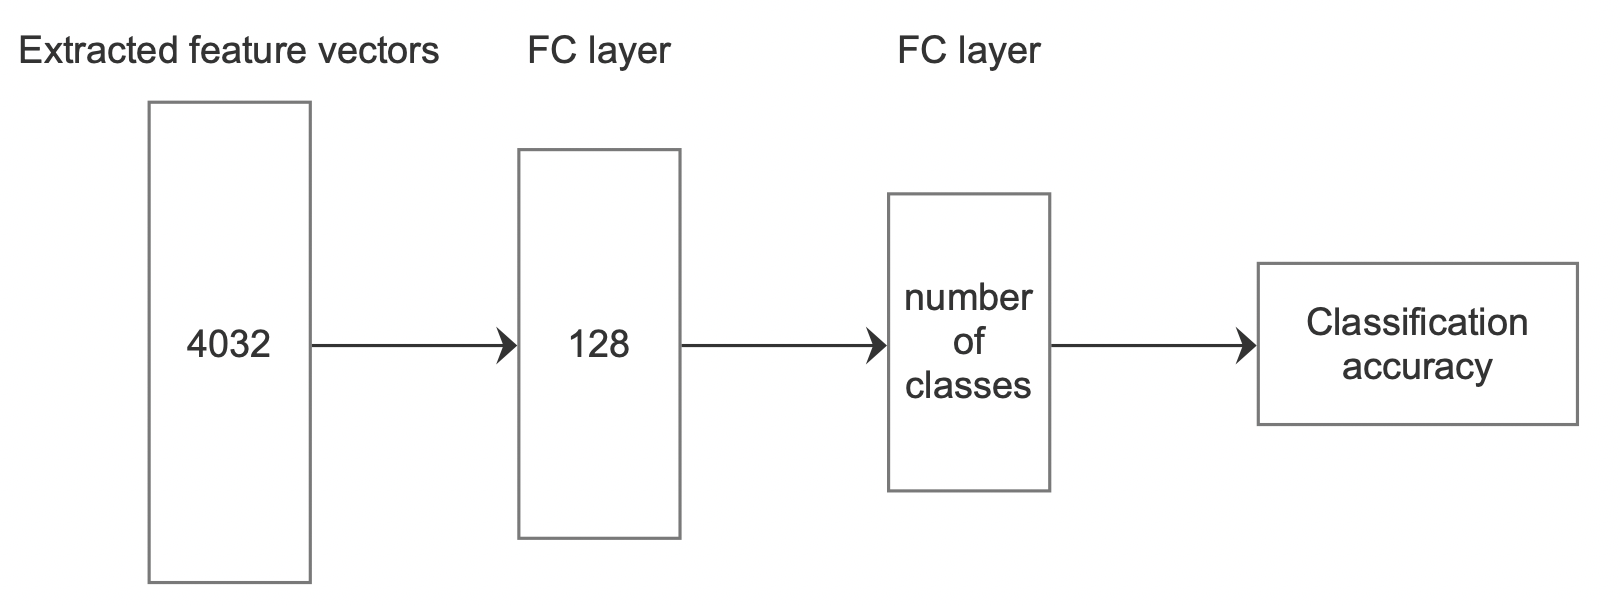
\includegraphics[width=0.9\textwidth]{src/compress_layer.png}
 \caption{Network structure to compress the extracted feature vectors.}
 \label{Fig.compress_layer}
 \end{figure}

\section{Difficulty Tuneable Algorithms}
Before presenting the evaluation plans, it should be noted that the algorithms described in \ref{ibalgorithm} are not perfect. POP and EGDIS are not deep learning based so the CNN may not work well with selected samples. Also, although CL is target hypothesis based algorithm, by keeping easy samples only may limit the performance that the network could achieve. Therefore, our first contribution is to modify these 

\subsection{Weighted Curriculum Learning}
Instead of selecting the top N samples based on CL scores, we use the scores as the sample weights just like the importance based methods. In this way, not only the easy samples are selected, some hard examples are also selected. Because we only select the subset once, this behaviour should be able to achieve higher accuracy if the network is good enough. However, if the network is not capable of handling these hard examples, then the accuracy may decay.


% WCL

\begin{algorithm}[H]
 \KwData{compressed 128-D feature vectors $M$}
  \KwIn{number of samples to select $m$, classification score for each sample $scores$, number of classes $n$}
 \KwOut{selected sample index by WCL}

$selected\_idx\_list = []$ \;

\ForEach{class label L}{
	scores = all sample scores with label L \;
	scores = scores / sum(scores) \;
	idx\_list = choose floor(m/n) samples based on scores \;
	selected\_idx\_list.append(idx\_list)) \;
}


\Return $selected\_idx\_list$ \;

\caption{WCL}
\end{algorithm}

\subsection{Boundary Based Weighted Curriculum Learning}
We also evaluated its EGDIS based variants which takes a propotion of EGDIS boundary samples so that we would have a higher chance selecting them. We keep class balance as a basic rule so we select 20\%, 40\% boundary samples if possible.

% BBWCL

\begin{algorithm}[H]
 \KwData{compressed 128-D feature vectors $M$}
  \KwIn{number of samples to select $m$, classification score for each sample $scores$, number of classes $n$, EGDIS boundary sample index list $egdis\_boundary\_index$, percent of boundary to select $p$}
 \KwOut{selected sample index by BWCL}

$selected\_idx\_list = []$ \;

\ForEach{class label L}{
	scores = all non-EGDIS sample scores with label L \;
	egdis\_boundary\_index\_L = all EGDIS boundary sample index with label L \;
	egdis\_idx = choose floor(m/n $\times$ p) samples from egdis\_boundary\_index\_L \;
	selected\_idx\_list.append(egdis\_idx)) \;
	
	scores = scores / sum(scores) \;
	idx\_list = choose floor(m/n$\times$ (1-p))
	 samples based on scores \;
	selected\_idx\_list.append(idx\_list)) \;
}


\Return $selected\_idx\_list$ \;

\caption{BWCL}
\end{algorithm}


\section{Evaluation Designs}
We have the following few experiments:
1. We use generated dataset to explore the intrinsic behaviour of these methods.
2. We use logistic regression to test all these methods. We also use the experiment results to decide how to select the subsets and the percentage range.
3. We select 3 subsets based on the test result of exp1, to run deep learning using incremental method. In total, we have experiment 9 network results on 5 datasets. We compare the experiment results and conclude the experiments.
